\documentclass[dvipdfmx]{standalone}
\usepackage{tikz}
\usepackage{pgfplots}
\pgfplotsset{compat=1.18}
\begin{document}
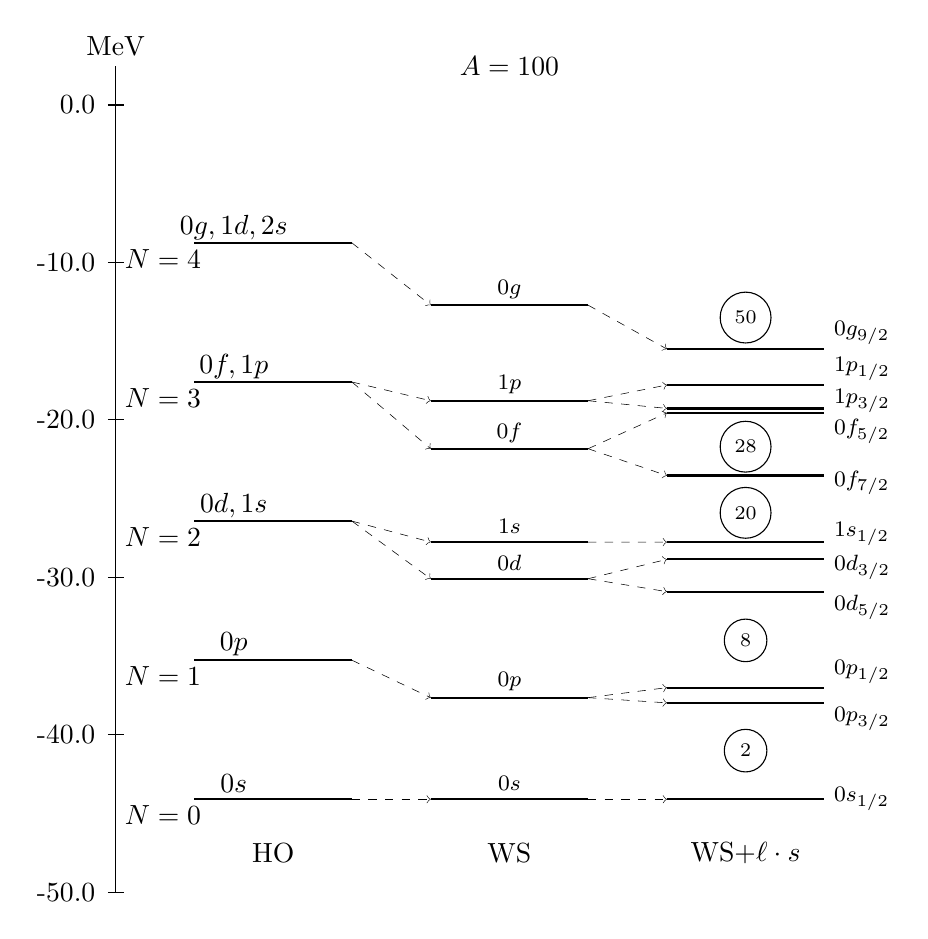
\begin{tikzpicture}

% 縦軸(エネルギーのスケール)
\draw (-0.5, -50/5) -- (-0.5, 0.5) node[above] {MeV};
\foreach \y/\text in {0.0/{0.0}, -10.0/{-10.0}, -20.0/{-20.0}, -30.0/{-30.0}, -40.0/{-40.0}, -50.0/{-50.0}} {
    \draw (-0.6, \y/5) -- (-0.4, \y/5) node[left] {\text\ \ \ };
}

% HOレベル(左側)
\node at (1.5, -50/5 +0.5) {HO};
\foreach \n/\y/\text in {
    4/-8.757/{$0g, 1d, 2s$},
    3/-17.591/{$0f, 1p$},
    2/-26.424/{$0d, 1s$},
    1/-35.257/{$0p$},
    0/-44.09/{$0s$}} {
    \node at (0.1, \y/5-0.2) {$N=\n$};
    \node at (1.0, \y/5+0.2) {\text};
    %横線の位置(x,y)
    \draw[thick] (0.5, \y/5) -- (2.5, \y/5);
}

% WSレベル(中央)
\node at (4.5, -50/5 +0.5) {WS};
\foreach \name/\y/\label in {
    0g/-12.713/58,
    1p/-18.782/40,
    0f/-21.829/34,
    1s/-27.754/20,
    0d/-30.084/18,
    0p/-37.636/8,
    0s/-44.09/2} {
    \node at (4.5, \y/5+0.2) {\footnotesize$\name$};
    \draw[thick] (3.5, \y/5) -- (5.5, \y/5);
}

% WS+ls(右側)
\node at (7.5, -50/5 +0.5) {WS+$\ell\cdot s$};
\foreach \name/\y/\label in {
    0g_{9/2}/-15.499/58,
    1p_{1/2}/-17.782/40,
    1p_{3/2}/-19.269/40,
    0f_{5/2}/-19.553/34,
    0f_{7/2}/-23.535/34,
    1s_{1/2}/-27.758/20,
    0d_{3/2}/-28.854/18,
    0d_{5/2}/-30.905/18,
    0p_{1/2}/-37.0/8,
    0p_{3/2}/-37.967/8,
    0s_{1/2}/-44.09/2} {
    \draw[thick] (6.5, \y/5) -- (8.5, \y/5);
}


\foreach \name/\y in {
    0g_{9/2}/-15.499,
    1p_{1/2}/-17.782,
    1p_{3/2}/-19.769,
    0f_{5/2}/-21.753,
    0f_{7/2}/-25.0,
    1s_{1/2}/-28.258,
    0d_{3/2}/-30.354,
    0d_{5/2}/-32.905,
    0p_{1/2}/-37.0,
    0p_{3/2}/-39.967,
    0s_{1/2}/-45.09} {
    \node[anchor=west] at (8.5, \y/5+0.2) {\footnotesize$\name$};
}

%矢印(HOからWSへの接続)
\foreach \yA/\yB in {
    -44.09/-44.09,
    -35.257/-37.636,
    -26.424/-30.084,
    -26.424/-27.754,
    -17.591/-21.829,
    -17.591/-18.782,
    -8.757/-12.713}{
    \draw[very thin,dashed,->] (2.5,\yA/5) -- (3.5,\yB/5);
}
%矢印(WSからws+ls)
\foreach \yA/\yB in {
    -44.09/-44.09,
    -37.636/-37.967,
    -37.636/-37.0,
    -30.084/-30.905,
    -30.084/-28.854,
    -27.754/-27.758,
    -21.829/-23.535,
    -21.829/-19.553,
    -18.782/-19.269,
    -18.782/-17.782,
    -12.713/-15.499}{
    \draw[very thin,dashed,->] (5.5,\yA/5) -- (6.5,\yB/5);
}
%魔法数
\foreach \y/\offset/\label in {
    -40/-0.2/2,
    -30/-0.8/8,
    -22/-0.78/20,
    -18/-0.74/28,
    -10/-0.7/50
} {
    \draw (7.5, \y/5 + \offset) node[draw, circle] {\scriptsize\label};
}


\node at (4.5,0.5) {$A=100$};
\end{tikzpicture}
\end{document}
